% !TeX spellcheck = en_US

\documentclass[document.tex]{subfiles}

\begin{document}
    \subsection{Introduction}
    
    \begin{frame}{Non-Linear Relationships}
        \begin{columns}
            \begin{column}{0.6\textwidth}
                \begin{itemize}
                    \item In the previous section we have evaluated \textbf{linear models} that are capable of predicting \textbf{continuous outcome} (regression; e.g., linear regression) and \textbf{discrete categorical outcome} (classification; e.g., logistic regression).
                    \item Unfortunately, these models tend to have a \textbf{high bias} especially if there is a \textbf{non-linear relationship} between the features and the target which is far more common in \textbf{real-world predictions tasks}.
                    \item And even though we have been able to model \textbf{quadratic or cubic relationships} by using the polynomials, the \textbf{true underlying relationship} might be much more complex especially when the \textbf{size of the feature space (complexity)} increases.
                \end{itemize}
            \end{column}
            \begin{column}{0.4\textwidth}
                \begin{figure}
                    \label{fig:non-linear-relationships}
                    \includegraphics[width=.8\textwidth, keepaspectratio]{figures/non-linear-relationships.pdf}
                \end{figure}
            \end{column}
        \end{columns}
    \end{frame}

    \begin{frame}{Decision Trees}
        \begin{columns}
            \begin{column}{0.6\textwidth}
                \begin{itemize}
                    \item Decision trees are \textbf{non-linear models} for \textbf{regression and classifications tasks} which try to \textbf{overcome the aforementioned problems} by generating \textbf{decision boundaries} that \textbf{bisect the space into smaller and smaller regions} in order to seperate the different classes.
                    \item The idea is to \textbf{construct a graphical representation} of all \textbf{possible solutions to a decision} based on \textbf{certain conditions} in form of a tree which starts with a \textbf{single root node} and then \textbf{branches off} into a number of further \textbf{decision nodes} based a on \textbf{splitting criterion} until a given \textbf{stop criterion} is reached.
                    \item Unlike many other models, decision trees are often considered as \textbf{white-box models} as they allow to \textbf{interpret the results and decisions} more easily due to their real-life analogy of \textbf{human decision-making}. 
                \end{itemize}
            \end{column}
            \begin{column}{0.4\textwidth}
                \begin{figure}
                    \label{fig:bisections}
                    \includegraphics[width=.8\textwidth, keepaspectratio]{figures/bisections.pdf}
                \end{figure}
            \end{column}
        \end{columns}
    \end{frame}

    \begin{frame}{Decision Tree Anatomy}
        \begin{columns}
            \begin{column}{0.5\textwidth}
                \begin{itemize}
                    \item \textbf{Root Node:} Entire population or sample, further gets divided into two or more homogeneous sets.
                    \item \textbf{Parent and Child Node:} Node which is divided into sub-nodes is called parent node, whereas sub-nodes are the child of parent node.
                    \item \textbf{Decision Node:} A sub-node that splits into further sub-nodes.
                    \item \textbf{Leaf/Terminal Node:} Nodes that do not split. Leaf node represents a classification or decision.
                    \item \textbf{Branch/Sub-Tree:} Sub-section of entire tree.
                \end{itemize}
            \end{column}
            \begin{column}{0.5\textwidth}
                \begin{figure}
                    \label{fig:decision-tree-anatomy}
                    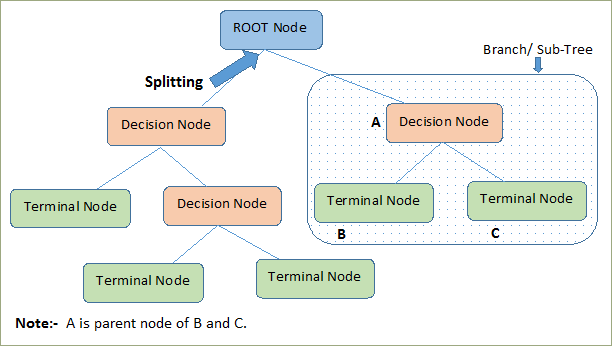
\includegraphics[width=\textwidth, keepaspectratio]{figures/external/decision-tree-anatomy.png}
                \end{figure}
            \end{column}
        \end{columns}
    \end{frame}

    \begin{frame}{Decision Tree Learning}
        \begin{itemize}
            \item The \textbf{construction of decision trees} based on training data is called \textbf{decision tree learning} in which the \textbf{training set} initially gets \textbf{partitioned into subsets} based on a \textbf{splitting criterion}. 
            \item For each derived subset the \textbf{process is repeated} in a recursive manner (\textbf{recursive partitioning}) until further splitting \textbf{no longer adds value} to the predictive capabilities of the model.
            \item This approach is called \textbf{top-down induction of decision trees} which is a \textbf{greedy algorithm} where at each stage the \textbf{locally optimal choice} is made in order to find a \textbf{global optimum}. 
            \item In order to construct decision trees, various algorithms exist like the \textbf{Iterative Dichotomiser 3 (ID3)} (Quinlan, 1986) or the \textbf{Classification And Regression Tree (CART)} (Breiman et al., 1984).
            \item In the following, the \textbf{ID3} will exemplarily be exercised, because it is a \textbf{very explanatory algorithm} which allows to clarify the \textbf{basic principles of decision tree learning} more easily. 
            \item Nevertheless, due to its \textbf{strong limitations}, the de-facto standard algorithm that is used in practice is \textbf{CART} which is implemented in almost all of the programming libraries available.
        \end{itemize}
    \end{frame}

    \begin{frame}{Introductory Example}
        Lets suppose we have been given a small dataset by a customer that contains categorized \textbf{measurements for vibration intensity and temperature} as well as \textbf{error and outage flags} for 14 machines (5 operable, 9 inoperable) whereas the outage flag here indicates whether or not a machine will fail within the next 7 days.

        \begin{table}
            \scalebox{0.8}{\begin{tabular}{crrrr}
\toprule
   i & Vibration Intensity & Error Indicator & Temperature & Outage Indicator \\
\midrule
   1 &                 low &              no &        high &               no \\
   2 &                 low &              no &         low &               no \\
   3 &                high &              no &        high &              yes \\
 ... &                 ... &             ... &         ... &              ... \\
  14 &              medium &             yes &         low &               no \\
\bottomrule
\end{tabular}
}
        \end{table}
        
        Another machine recently showed \textbf{medium vibration with low temperature and negative error indicator}. As this specific example is not in the dataset, our job now is to \textbf{learn a decision tree model} that is capable of \textbf{predicting whether or not this machine will fail within the next 7 days}.
        
        \small{\href{https://nbviewer.jupyter.org/github/saschaschworm/big-data-and-data-science/blob/master/notebooks/demos/outage-decision-tree-learning.ipynb}{\textsc{\textbf{$\rightarrow$ open notebook in github}}}}
    \end{frame}

    \begin{frame}{Categorical Encoding}
        \begin{itemize}
            \item Many machine learning models and algorithms require \textbf{categorical features} to be transformed into their \textbf{numerical representations} in order to work but as with many other aspects in data science there is \textbf{no single answer} in how to approach this problem properly.
            \item Two \textbf{popular approaches} that are commonly used when preprocessing categorical features are called \textbf{label encoding} and \textbf{one-hot encoding} where each approach has it own \textbf{strengths and weaknesses} that have \textbf{potential impact on both outcome and accuracy}.
            \item In the following we will take a close look on how label and one-hot encoding works, what \textbf{potential problems} may occur and how we can implement them into our \textbf{data preprocessing pipeline}.
        \end{itemize}
    \end{frame}

    \begin{frame}{Label Encoding}
        \textbf{Label encoding} simply \textbf{encodes the labels of a categorical feature numerically} with a value between $0$ and $N-1$ where $N$ is the number of classes in this categorical feature.
        
        \begin{center}
            \begin{minipage}{0.4\textwidth}
                \begin{table}
                    \scalebox{0.8}{\begin{tabular}{crrrr}
\toprule
   i & vibration & error & temperature & outage \\
\midrule
   1 &       low &    no &        high &     no \\
   2 &       low &    no &         low &     no \\
   3 &      high &    no &        high &    yes \\
 ... &       ... &   ... &         ... &    ... \\
  14 &    medium &   yes &         low &     no \\
\bottomrule
\end{tabular}
}
                \end{table}
            \end{minipage}%
            \begin{minipage}{0.4\textwidth}
                \begin{table}
                    \scalebox{0.8}{\begin{tabular}{crrrr}
\toprule
   i & vibration & error & temperature & outage \\
\midrule
   1 &         1 &     0 &           0 &     no \\
   2 &         1 &     0 &           1 &     no \\
   3 &         0 &     0 &           0 &    yes \\
 ... &       ... &   ... &         ... &    ... \\
  14 &         2 &     1 &           1 &     no \\
\bottomrule
\end{tabular}
}
                \end{table}
            \end{minipage}
        \end{center}
        
        However, depending on the data, label encoding introduces a problem as it brings a \textbf{natural ordering for different classes}. When there is no actual relation, a model will \textbf{misunderstand the data} to be in some kind of order $0 < 1 < 2$ which will lead to poor performance - especially for models that \textbf{weight features} like linear or logistic regression does.
    \end{frame}

    \begin{frame}{One-Hot Encoding}
        We can avoid learning a model some kind of order when it is clearly not present by using \textbf{one-hot-encoding} which \textbf{removes a label encoded variable} and \textbf{adds a new binary variable for each unique integer value} especially for mode

        \begin{center}
            \begin{minipage}{0.4\textwidth}
                \begin{table}
                    \scalebox{0.8}{\begin{tabular}{crrrr}
\toprule
   i & vibration & error & temperature & outage \\
\midrule
   1 &       low &    no &        high &     no \\
   2 &       low &    no &         low &     no \\
   3 &      high &    no &        high &    yes \\
 ... &       ... &   ... &         ... &    ... \\
  14 &    medium &   yes &         low &     no \\
\bottomrule
\end{tabular}
}
                \end{table}
            \end{minipage}%
            \begin{minipage}{0.6\textwidth}
                \begin{table}
                    \scalebox{0.8}{\begin{tabular}{crrrrrrrr}
\toprule
   i & vibration\_low & vibration\_medium & error\_yes &  ... & outage \\
\midrule
   1 &             1 &                0 &         0 &  ... &     no \\
   2 &             1 &                0 &         0 &  ... &     no \\
   3 &             0 &                0 &         0 &  ... &    yes \\
 ... &           ... &              ... &       ... &  ... &    ... \\
  14 &             0 &                1 &         1 &  ... &     no \\
\bottomrule
\end{tabular}
}
                \end{table}
            \end{minipage}
        \end{center}
    
        The problem with one-hot encoding is that the \textbf{feature space} can blow up quickly. If there is \textbf{high cardinality} in the \textbf{categorical features} relative to the amount of data, models will be unable to learn efficiently. This problem is called the \textbf{curse of dimensionality} and can lead to \textbf{overfitting}.
    \end{frame}
    
    \begin{frame}{Python Implementation: Label and One-Hot Encoding}
        \lstinputlisting[language=Python, style=material]{snippets/categorical-encoding.py}
    \end{frame}
    
    \subsection{Iterative Dichotomiser 3 (ID3)}
    
   	\begin{frame}{Iterative Dichotomiser 3 (ID3)}
        \begin{itemize}
            \item The ID3 iteratively \textbf{divides features into two groups} to construct a tree (\textbf{dichotomisation}). The first group contains the \textbf{most dominant feature} and the other group contains all other features. 
            \item The \textbf{most dominant feature (or best split)} is found by calculating the \textbf{entropy} and \textbf{information gains} of each feature. The \textbf{best feature} is the one which gives the \textbf{maximum information gain} (\textbf{splitting criterion}) and therefore partitions the instances in a given subset best according to their target label.
            \item Then, the \textbf{most dominant feature} is put on the tree as \textbf{decision node} and after that, entropy and information gains are again calculated among the other attributes.
            \item This \textbf{process is repeated} for each branch until \textbf{every attribute has already been included} along this pass through tree or the \textbf{entropy is zero}.
        \end{itemize}
    \end{frame}
    
    \begin{frame}{Entropy}
        \begin{itemize}
            \item A measure commonly used in \textbf{information theory} to characterize the \textbf{(im)purity} of instances in a dataset is called \textbf{entropy} $H(S)$ which is defined as:
            $$
            H(S) = \sum_{c \in C}-p(c)log_2p(c),
            $$
            where $S$ is the current dataset for which entropy is being calculated, $C$ is the set of classes in $S$ and $p(c)$ is the proportion of the number of elements in class $c$ to the number of elements in dataset $S$.
            \item This means for a \textbf{binary classifcation problem}, that if \textbf{all instances in a dataset are positive or all are negative} then entropy will be \textbf{zero}. If \textbf{half examples are of positive class and half are of negative class} then entropy is \textbf{one}.
        \end{itemize}
    \end{frame}
    
    \begin{frame}{Information Gain}
        \begin{itemize}
            \item The \textbf{optimal attribute for splitting} the a tree node is the one with the \textbf{most entropy reduction}. To measure this expected entropy reduction, the \textbf{information gain} need to be calculated which is based on the \textbf{decrease in entropy after a dataset is split on an attribute}. 
            \item The information gain $IG(A, S)$ is defined as:
            $$
            IG(A, S) = H(S) - \sum_{t \in T} \frac{|t|}{|S|}H(t),
            $$
            where $H(S)$ is the entropy of dataset $S$, $T$ are the subsets created from splitting $S$ by attribute $A$, $\frac{|t|}{|S|}$ is the proportion of the number of instances in $t$ to the number of instances in dataset $S$ and $H(t)$ is the entropy of subset $t$.
        \end{itemize}
    \end{frame}    
    
    \begin{frame}{Sample ID3 Tree Construction (1st Iteration) I/V}
        \begin{columns}
            \begin{column}{0.4\textwidth}
                \begin{table}
                    \caption*{\footnotesize Sample $S$ \normalsize}
                    \vspace*{-2mm}					
                    \scalebox{0.7}{
                        \begin{tabular}{llll}
                            \toprule
                            \textbf{vibration} & \textbf{error} & \textbf{temperature} & \textbf{outage} \\
                            \midrule
                            \rowcolor{LightRed}
                            low &    no &        high &     no \\
                            \rowcolor{LightRed}
                            low &    no &         low &     no \\
                            \rowcolor{LightGreen}
                            high &    no &        high &    yes \\
                            \rowcolor{LightGreen}
                            medium &    no &        high &    yes \\
                            \rowcolor{LightGreen}
                            medium &   yes &        high &    yes \\
                            \rowcolor{LightRed}
                            medium &   yes &         low &     no \\
                            \rowcolor{LightGreen}
                            high &   yes &         low &    yes \\
                            \rowcolor{LightRed}
                            low &    no &        high &     no \\
                            \rowcolor{LightGreen}
                            low &   yes &        high &    yes \\
                            \rowcolor{LightGreen}
                            medium &   yes &        high &    yes \\
                            \rowcolor{LightGreen}
                            low &   yes &         low &    yes \\
                            \rowcolor{LightGreen}
                            high &    no &         low &    yes \\
                            \rowcolor{LightGreen}
                            high &   yes &        high &    yes \\
                            \rowcolor{LightRed}
                            medium &   yes &         low &     no \\
                            \bottomrule
                        \end{tabular}
                    }
                \end{table}
            \end{column}
            \begin{column}{0.6\textwidth}
                \begin{alignat*}{3}
                H(S) &= -\frac{9}{14}log_2(\frac{9}{14}) - \frac{5}{14}log_2(\frac{5}{14}) &&= 0.94
                \end{alignat*}
            \end{column}
        \end{columns}
    \end{frame}

    \begin{frame}{Sample ID3 Tree Construction (1st Iteration) II/V}
        \begin{columns}
            \begin{column}{0.4\textwidth}
                \begin{table}
                    \caption*{\footnotesize Attribute $A=VIBRATION$, Sample $S_L$ \normalsize}
                    \vspace*{-2mm}	
                    \scalebox{0.7}{
                        \begin{tabular}{llll}
                            \toprule
                            \textbf{vibration} & \textbf{error} & \textbf{temperature} & \textbf{outage} \\
                            \midrule
                            \rowcolor{LightRed}
                            low &    no &        high &     no \\
                            \rowcolor{LightRed}
                            low &    no &         low &     no \\
                            \rowcolor{LightRed}
                            low &    no &        high &     no \\
                            \rowcolor{LightGreen}
                            low &   yes &        high &    yes \\
                            \rowcolor{LightGreen}
                            low &   yes &         low &    yes \\
                            \bottomrule
                        \end{tabular}
                    }
                \end{table}
                \vspace*{-6mm}
                \begin{table}
                    \caption*{\footnotesize Attribute $A=VIBRATION$, Sample $S_M$ \normalsize}
                    \vspace*{-2mm}	
                    \scalebox{0.7}{
                        \begin{tabular}{llll}
                            \toprule
                            \textbf{vibration} & \textbf{error} & \textbf{temperature} & \textbf{outage} \\
                            \midrule
                            \rowcolor{LightGreen}
                            medium &    no &        high &    yes \\
                            \rowcolor{LightGreen}
                            medium &   yes &        high &    yes \\
                            \rowcolor{LightRed}
                            medium &   yes &         low &     no \\
                            \rowcolor{LightGreen}
                            medium &   yes &        high &    yes \\
                            \rowcolor{LightRed}
                            medium &   yes &         low &     no \\
                            \bottomrule
                        \end{tabular}
                    }
                \end{table}
                \vspace*{-6mm}
                \begin{table}
                    \caption*{\footnotesize Attribute $A=VIBRATION$, Sample $S_H$ \normalsize}
                    \vspace*{-2mm}	
                    \scalebox{0.7}{
                        \begin{tabular}{llll}
                            \toprule
                            \textbf{vibration} & \textbf{error} & \textbf{temperature} & \textbf{outage} \\
                            \midrule
                            \rowcolor{LightRed}
                            \rowcolor{LightGreen}
                            high &    no &        high &    yes \\
                            \rowcolor{LightGreen}
                            high &   yes &         low &    yes \\
                            \rowcolor{LightGreen}
                            high &    no &         low &    yes \\
                            \rowcolor{LightGreen}
                            high &   yes &        high &    yes \\
                            \bottomrule
                        \end{tabular}
                    }
                \end{table}
            \end{column}
            \begin{column}{0.6\textwidth}
                \begin{alignat*}{3}
                    H(S) &= 0.94 \\\\
                    H(S_L) &= -\frac{2}{5}log_2(\frac{2}{5}) - \frac{3}{5}log_2(\frac{3}{5}) &&= 0.97 \\
                    H(S_M) &= -\frac{3}{5}log_2(\frac{3}{5}) - \frac{2}{5}log_2(\frac{2}{5}) &&= 0.97 \\
                    H(S_H) &= -\frac{4}{4}log_2(\frac{4}{4}) - \frac{0}{0}log_2(\frac{0}{0}) &&= 0.0 \\\\
                    IG(S, A) &= 0.94 - \frac{5}{14} 0.97 - \frac{5}{14} 0.97 - \frac{4}{14} 0.0 &&= 0.25
                \end{alignat*}
            \end{column}
        \end{columns}
    \end{frame}

    \begin{frame}{Sample ID3 Tree Construction (1st Iteration) III/V}
        \begin{columns}
            \begin{column}{0.4\textwidth}
                \begin{table}
                    \caption*{\footnotesize Attribute $A=ERROR$, Sample $S_N$ \normalsize}
                    \vspace*{-2mm}
                    \scalebox{0.7}{
                        \begin{tabular}{llll}
                            \toprule
                            \textbf{vibration} & \textbf{error} & \textbf{temperature} & \textbf{outage} \\
                            \midrule
                            \rowcolor{LightRed}
                            low &    no &        high &     no \\
                            \rowcolor{LightRed}
                            low &    no &         low &     no \\
                            \rowcolor{LightGreen}
                            high &    no &        high &    yes \\
                            \rowcolor{LightGreen}
                            medium &    no &        high &    yes \\
                            \rowcolor{LightRed}
                            low &    no &        high &     no \\
                            \rowcolor{LightGreen}
                            high &    no &         low &    yes \\
                            \bottomrule
                        \end{tabular}
                    }
                \end{table}
                \vspace*{-6mm}
                \begin{table}
                    \caption*{\footnotesize Attribute $A=ERROR$, Sample $S_Y$ \normalsize}
                    \vspace*{-2mm}
                    \scalebox{0.7}{
                        \begin{tabular}{llll}
                            \toprule
                            \textbf{vibration} & \textbf{error} & \textbf{temperature} & \textbf{outage} \\
                            \midrule
                            \rowcolor{LightGreen}
                            medium &   yes &        high &    yes \\
                            \rowcolor{LightRed}
                            medium &   yes &         low &     no \\
                            \rowcolor{LightGreen}
                            high &   yes &         low &    yes \\
                            \rowcolor{LightGreen}
                            low &   yes &        high &    yes \\
                            \rowcolor{LightGreen}
                            medium &   yes &        high &    yes \\
                            \rowcolor{LightGreen}
                            low &   yes &         low &    yes \\
                            \rowcolor{LightGreen}
                            high &   yes &        high &    yes \\
                            \rowcolor{LightRed}
                            medium &   yes &         low &     no \\
                            \bottomrule
                        \end{tabular}
                    }
                \end{table}
            \end{column}
            \begin{column}{0.6\textwidth}
                \begin{alignat*}{3}
                    H(S) &= 0.94 \\
                    IG(S, A_{VIBRATION}) &= 0.25 \\\\
                    H(S_N) &= -\frac{3}{6}log_2(\frac{3}{6}) - \frac{3}{6}log_2(\frac{3}{6}) &&= 1.0 \\
                    H(S_Y) &= -\frac{6}{8}log_2(\frac{6}{8}) - \frac{2}{8}log_2(\frac{2}{8}) &&= 0.81 \\\\
                    IG(S, A) &= 0.94 - \frac{6}{14} 1.00 - \frac{8}{14} 0.81 &&= 0.05
                \end{alignat*}
            \end{column}
        \end{columns}
    \end{frame}	
                
    \begin{frame}{Sample ID3 Tree Construction (1st Iteration) IV/V}
        \begin{columns}
            \begin{column}{0.4\textwidth}
                \begin{table}
                    \caption*{\footnotesize Attribute $A=TEMPERATURE$, Sample $S_H$ \normalsize}
                    \vspace*{-2mm}
                    \scalebox{0.7}{
                        \begin{tabular}{llll}
                            \toprule
                            \textbf{vibration} & \textbf{error} & \textbf{temperature} & \textbf{outage} \\
                            \midrule
                            \rowcolor{LightRed}
                            low &    no &        high &     no \\
                            \rowcolor{LightGreen}
                            high &    no &        high &    yes \\
                            \rowcolor{LightGreen}
                            medium &    no &        high &    yes \\
                            \rowcolor{LightGreen}
                            medium &   yes &        high &    yes \\
                            \rowcolor{LightRed}
                            low &    no &        high &     no \\
                            \rowcolor{LightGreen}
                            low &   yes &        high &    yes \\
                            \rowcolor{LightGreen}
                            medium &   yes &        high &    yes \\
                            \rowcolor{LightGreen}
                            high &   yes &        high &    yes \\
                            \bottomrule
                        \end{tabular}
                    }
                \end{table}
                \vspace*{-6mm}
                \begin{table}
                    \caption*{\footnotesize Attribute $A=TEMPERATURE$, Sample $S_L$ \normalsize}
                    \vspace*{-2mm}
                    \scalebox{0.7}{
                        \begin{tabular}{llll}
                            \toprule
                            \textbf{vibration} & \textbf{error} & \textbf{temperature} & \textbf{outage} \\
                            \midrule
                            \rowcolor{LightRed}
                            low &    no &         low &     no \\
                            \rowcolor{LightRed}
                            medium &   yes &         low &     no \\
                            \rowcolor{LightGreen}
                            high &   yes &         low &    yes \\
                            \rowcolor{LightGreen}
                            low &   yes &         low &    yes \\
                            \rowcolor{LightGreen}
                            high &    no &         low &    yes \\
                            \rowcolor{LightRed}
                            medium &   yes &         low &     no \\
                            \bottomrule
                        \end{tabular}
                    }
                \end{table}
            \end{column}
            \begin{column}{0.6\textwidth}
                \begin{align*}
                    H(S) &= 0.94 \\
                    IG(S, A_{VIBRATION}) &= 0.25 \text{ (Highest IG, Best Split)} \\
                    IG(S, A_{ERROR}) &= 0.05 \\\\
                    H(S_H) &= -\frac{6}{8}log_2(\frac{6}{8}) - \frac{2}{8}log_2(\frac{2}{8}) &&= 0.81 \\
                    H(S_L) &= -\frac{3}{6}log_2(\frac{3}{6}) - \frac{3}{6}log_2(\frac{3}{6}) &&= 1.0 \\\\
                    IG(S, A) &= 0.94 - \frac{8}{14} 0.81 - \frac{6}{14} 1.0 &&= 0.05
                \end{align*}
            \end{column}
        \end{columns}
    \end{frame}	

    \begin{frame}{Sample ID3 Tree Construction (1st Iteration) V/V}
        \begin{figure}
            \includegraphics[height=0.8\textheight, keepaspectratio]{figures/outages-idthree-man-1.pdf}
        \end{figure}
    \end{frame}
    
    \begin{frame}{Sample ID3 Tree Construction (2nd Iteration) I/III}
        \begin{columns}
            \begin{column}{0.4\textwidth}
                \begin{table}
                    \caption*{\footnotesize Sample $S$ \normalsize}
                    \vspace*{-2mm}
                    \scalebox{0.7}{
                        \begin{tabular}{llll}
                            \toprule
                            \textbf{\sout{vibration}} & \textbf{error} & \textbf{temperature} & \textbf{outage} \\
                            \midrule
                            \rowcolor{LightRed}
                            low &    no &        high &     no \\
                            \rowcolor{LightRed}
                            low &    no &         low &     no \\
                            \rowcolor{LightRed}
                            low &    no &        high &     no \\
                            \rowcolor{LightGreen}
                            low &   yes &        high &    yes \\
                            \rowcolor{LightGreen}
                            low &   yes &         low &    yes \\
                            \bottomrule
                        \end{tabular}
                    }
                \end{table}
                \vspace*{-6mm}
                \begin{table}
                    \caption*{\footnotesize Attribute $A=TEMPERATURE$, Sample $S_H$ \normalsize}
                    \vspace*{-2mm}
                    \scalebox{0.7}{
                        \begin{tabular}{llll}
                            \toprule
                            \textbf{\sout{vibration}} & \textbf{error} & \textbf{temperature} & \textbf{outage} \\
                            \midrule
                            \rowcolor{LightRed}
                            low &    no &        high &     no \\
                            \rowcolor{LightRed}
                            low &    no &        high &     no \\
                            \rowcolor{LightGreen}
                            low &   yes &        high &    yes \\
                            \bottomrule
                        \end{tabular}
                    }
                \end{table}
                \vspace*{-6mm}
                \begin{table}
                    \caption*{\footnotesize Attribute $A=TEMPERATURE$, Sample $S_L$ \normalsize}
                    \vspace*{-2mm}
                    \scalebox{0.7}{
                        \begin{tabular}{llll}
                            \toprule
                            \textbf{\sout{vibration}} & \textbf{error} & \textbf{temperature} & \textbf{outage} \\
                            \midrule
                            \rowcolor{LightRed}
                            low &    no &         low &     no \\
                            \rowcolor{LightGreen}
                            low &   yes &         low &    yes \\
                            \bottomrule
                        \end{tabular}
                    }
                \end{table}
            \end{column}
            \begin{column}{0.6\textwidth}
                \begin{alignat*}{3}
                    H(S) &= -\frac{2}{5}log_2(\frac{2}{5}) - \frac{3}{5}log_2(\frac{3}{5}) &&= 0.97 \\\\
                    H(S_H) &= -\frac{1}{3}log_2(\frac{1}{3}) - \frac{2}{3}log_2(\frac{2}{3}) &&= 0.92 \\
                    H(S_L) &= -\frac{1}{2}log_2(\frac{1}{2}) - \frac{1}{2}log_2(\frac{1}{2}) &&= 1.0 \\\\
                    IG(S, A) &= 0.97 - \frac{3}{5} 0.92 - \frac{2}{5} 1.0 &&= 0.02
                \end{alignat*}
            \end{column}
        \end{columns}
    \end{frame}
    
    \begin{frame}{Sample ID3 Tree Construction (2nd Iteration) II/III}
        \begin{columns}
            \begin{column}{0.4\textwidth}
                \begin{table}
                    \caption*{\footnotesize Sample $S$ \normalsize}
                    \vspace*{-2mm}
                    \scalebox{0.7}{
                        \begin{tabular}{llll}
                            \toprule
                            \textbf{\sout{vibration}} & \textbf{error} & \textbf{temperature} & \textbf{outage} \\
                            \midrule
                            \rowcolor{LightRed}
                            low &    no &        high &     no \\
                            \rowcolor{LightRed}
                            low &    no &         low &     no \\
                            \rowcolor{LightRed}
                            low &    no &        high &     no \\
                            \rowcolor{LightGreen}
                            low &   yes &        high &    yes \\
                            \rowcolor{LightGreen}
                            low &   yes &         low &    yes \\
                            \bottomrule
                        \end{tabular}
                    }
                \end{table}
                \vspace*{-6mm}
                \begin{table}
                    \caption*{\footnotesize Attribute $A=ERROR$, Sample $S_N$ \normalsize}
                    \vspace*{-2mm}
                    \scalebox{0.7}{
                        \begin{tabular}{llll}
                            \toprule
                            \textbf{\sout{vibration}} & \textbf{error} & \textbf{temperature} & \textbf{outage} \\
                            \midrule
                            \rowcolor{LightRed}
                            low &    no &        high &     no \\
                            \rowcolor{LightRed}
                            low &    no &         low &     no \\
                            \rowcolor{LightRed}
                            low &    no &        high &     no \\
                            \bottomrule
                        \end{tabular}
                    }
                \end{table}
                \vspace*{-6mm}
                \begin{table}
                    \caption*{\footnotesize Attribute $A=ERROR$, Sample $S_Y$ \normalsize}
                    \vspace*{-2mm}
                    \scalebox{0.7}{
                        \begin{tabular}{llll}
                            \toprule
                            \textbf{\sout{vibration}} & \textbf{error} & \textbf{temperature} & \textbf{outage} \\
                            \midrule
                            \rowcolor{LightGreen}
                            low &   yes &        high &    yes \\
                            \rowcolor{LightGreen}
                            low &   yes &         low &    yes \\
                            \bottomrule
                        \end{tabular}
                    }
                \end{table}
            \end{column}
            \begin{column}{0.6\textwidth}
                \begin{alignat*}{3}
                    H(S) &= 0.97 \\
                    IG(S, A_{TEMPERATURE}) &= 0.02 \\\\
                    H(S_N) &= -\frac{0}{3}log_2(\frac{0}{3}) - \frac{3}{3}log_2(\frac{3}{3}) &&= 0.0 \\
                    H(S_Y) &= -\frac{2}{2}log_2(\frac{2}{2}) - \frac{0}{2}log_2(\frac{0}{2}) &&= 0.0 \\\\
                    \text{Leaf found: } ERROR_{NO} &\Rightarrow NO \\
                    \text{Leaf found: } ERROR_{YES} &\Rightarrow YES
                \end{alignat*}
            \end{column}
        \end{columns}
    \end{frame}
    
    \begin{frame}{Sample ID3 Tree Construction (2nd Iteration) III/III}
        \begin{figure}
            \includegraphics[height=0.8\textheight, keepaspectratio]{figures/outages-idthree-man-2.pdf}
        \end{figure}
    \end{frame}
    
    \begin{frame}{Sample ID3 Tree Construction (3rd Iteration) I/II}
        \begin{columns}
            \begin{column}{0.4\textwidth}
                \begin{table}
                    \caption*{\footnotesize Sample $S$ \normalsize}
                    \vspace*{-2mm}
                    \scalebox{0.7}{
                        \begin{tabular}{llll}
                            \toprule
                            \textbf{\sout{vibration}} & \textbf{\sout{error}} & \textbf{temperature} & \textbf{outage} \\
                            \midrule
                            \rowcolor{LightGreen}
                            medium &    no &        high &    yes \\
                            \rowcolor{LightGreen}
                            medium &   yes &        high &    yes \\
                            \rowcolor{LightRed}
                            medium &   yes &         low &     no \\
                            \rowcolor{LightGreen}
                            medium &   yes &        high &    yes \\
                            \rowcolor{LightRed}
                            medium &   yes &         low &     no \\
                            \bottomrule
                        \end{tabular}
                    }
                \end{table}
                \vspace*{-6mm}
                \begin{table}
                    \caption*{\footnotesize Attribute $A=TEMPERATURE$, Sample $S_H$ \normalsize}
                    \vspace*{-2mm}
                    \scalebox{0.7}{
                        \begin{tabular}{llll}
                            \toprule
                            \textbf{\sout{vibration}} & \textbf{\sout{error}} & \textbf{temperature} & \textbf{outage} \\
                            \midrule
                            \rowcolor{LightGreen}
                            medium &    no &        high &    yes \\
                            \rowcolor{LightGreen}
                            medium &   yes &        high &    yes \\
                            \rowcolor{LightGreen}
                            medium &   yes &        high &    yes \\
                            \bottomrule
                        \end{tabular}
                    }
                \end{table}
                \vspace*{-6mm}
                \begin{table}
                    \caption*{\footnotesize Attribute $A=TEMPERATURE$, Sample $S_L$ \normalsize}
                    \vspace*{-2mm}
                    \scalebox{0.7}{
                        \begin{tabular}{llll}
                        \toprule
                            \textbf{\sout{vibration}} & \textbf{\sout{error}} & \textbf{temperature} & \textbf{outage} \\
                            \midrule
                            \rowcolor{LightRed}
                            medium &   yes &         low &     no \\
                            \rowcolor{LightRed}
                            medium &   yes &         low &     no \\
                            \bottomrule
                        \end{tabular}
                    }
                \end{table}
            \end{column}
            \begin{column}{0.6\textwidth}
                \begin{alignat*}{3}
                    H(S) &= -\frac{3}{5}log_2(\frac{3}{5}) - \frac{2}{5}log_2(\frac{2}{5}) &&= 0.97 \\\\
                    H(S_N) &= -\frac{3}{3}log_2(\frac{3}{3}) - \frac{3}{3}log_2(\frac{3}{3}) &&= 0.0 \\
                    H(S_Y) &= -\frac{0}{2}log_2(\frac{0}{2}) - \frac{2}{2}log_2(\frac{2}{2}) &&= 0.0 \\\\
                    \text{Leaf found: } TEMPERATURE_{HIGH} &\Rightarrow YES \\
                    \text{Leaf found: } TEMPERATURE_{LOW} &\Rightarrow NO
                \end{alignat*}
            \end{column}
        \end{columns}
    \end{frame}
        
    \begin{frame}{Sample ID3 Tree Construction (3rd Iteration) II/II}
        \begin{figure}
            \includegraphics[height=0.8\textheight, keepaspectratio]{figures/outages-idthree-man-3.pdf}
        \end{figure}
    \end{frame}
        
    \begin{frame}{Sample ID3 Tree Construction (4th Iteration) I/II}
        \begin{columns}
            \begin{column}{0.4\textwidth}
                \begin{table}
                    \caption*{\footnotesize Sample $S$ \normalsize}
                    \vspace*{-2mm}
                    \scalebox{0.7}{
                        \begin{tabular}{llll}
                            \toprule
                            \textbf{\sout{vibration}} & \textbf{\sout{error}} & \textbf{\sout{temperature}} & \textbf{outage} \\
                            \midrule
                            \rowcolor{LightRed}
                            \rowcolor{LightGreen}
                            high &    no &        high &    yes \\
                            \rowcolor{LightGreen}
                            high &   yes &         low &    yes \\
                            \rowcolor{LightGreen}
                            high &    no &         low &    yes \\
                            \rowcolor{LightGreen}
                            high &   yes &        high &    yes \\
                            \bottomrule
                        \end{tabular}
                    }
                \end{table}
            \end{column}
            \begin{column}{0.6\textwidth}
                \begin{alignat*}{3}
                    H(S) &= -\frac{4}{4}log_2(\frac{4}{4}) - \frac{0}{0}log_2(\frac{0}{0}) &&= 0 \\\\
                    \text{Leaf found: } VIBRATION_{HIGH} &\Rightarrow YES \\
                \end{alignat*}
            \end{column}
        \end{columns}
    \end{frame}
    
    \begin{frame}{Sample ID3 Tree Construction (4th Iteration) II/II}
        \begin{figure}
            \includegraphics[height=0.8\textheight, keepaspectratio]{figures/outages-idthree-man-4.pdf}
        \end{figure}
    \end{frame}

    \begin{frame}{Python Implementation: Iterative Dichotomiser 3 I/III}
        \lstinputlisting[language=Python, style=material]{snippets/outtage-iterative-dichotomiser-1.py}
    \end{frame}

    \begin{frame}{Python Implementation: Iterative Dichotomiser 3 II/III}
        \lstinputlisting[language=Python, style=material]{snippets/outtage-iterative-dichotomiser-2.py}
    \end{frame}

    \begin{frame}{Python Implementation: Iterative Dichotomiser 3 III/III}
        \lstinputlisting[language=Python, style=material]{snippets/outtage-iterative-dichotomiser-3.py}

        A machine with \textbf{medium vibration, low temperature and negative error indicator} is \textbf{predicted not to fail within the next 7 days} with a \textbf{probability estimate of 100\%}.
    \end{frame}

    \begin{frame}{Predictive Maintenance Problem Result (ID3}
        \begin{figure}
            \label{fig:outages-idthree-decision-tree}
            \includegraphics[height=0.8\textheight, keepaspectratio]{figures/outages-idthree-decision-tree.pdf}
        \end{figure}
    \end{frame}

    \stepcounter{openexercise}
    \begin{frame}{Open Exercise \arabic{openexercise}}
        What would be a good classification metric to evaluate the performance of our decision tree model in predicting machine failures?
        \note{
            As the dataset is \textbf{slightly unbalanced}, the accuracy might not be good performance indicator. Both \textbf{not predicting actual machine failures and predicting false machine failures lead to a costly downtime} thus making both \textbf{precision and recall unuseful and the \textbf{F1 score} more appropriate}. 

        }
    \end{frame}

    \stepcounter{openexercise}
    \begin{frame}{Open Exercise \arabic{openexercise}}
        By using the following snippet we are able to calculate an average \textbf{F1 score with a 4-fold cross-validation}:

        \lstinputlisting[language=Python, style=material]{snippets/outage-idthree-evaluation.py}

        For what reason you should be alarmed?
        \note{
            There is in fact \textbf{no training error} which means that the decision tree has been able to \textbf{perfectly fit the data} which is rather unusual - especially when the \textbf{test error is higher than the training error}. It seems like the model is \textbf{overfitting} the data.

        }
    \end{frame}

    \begin{frame}[fragile]{Regression Counterpart}
        Of course, decision trees are also suitable for \textbf{regression problems} by using a \verb|DecisionTreeRegressor| instead of a \verb|DecisionTreeClassifier| like follows:

        \begin{lstlisting}[language=Python, style=material]
# Additional Import Definitions
from sklearn.tree import DecisionTreeRegressor

# Model Initialization
model = DecisionTreeRegressor(**hyperparams)
        \end{lstlisting}

        A decision tree for regression problems uses the \textbf{mean squared error} to measure the quality of a split and tries to minimizes the \textbf{L2 loss function} using the mean of each terminal node. To incorporate this, remember to set the hyperparameter \verb|criterion| to \verb|mse| instead of \verb|entropy|.
    \end{frame}

    \subsection{Random Forest}

    \begin{frame}{Ensemble Model}
        \begin{columns}
            \begin{column}{.6\textwidth}
                \begin{itemize}
                    \item The reason the \textbf{decision trees are prone to overfitting} is because it has \textbf{unlimited flexibility}, as it can \textbf{keep growing until it has exactly one leaf node for every single observation}, perfectly classifying all of them and thus having a \textbf{low bias}.
                    \item The objective of a any machine learning model is to \textbf{generalize well to new data it has never seen before}, but decision trees learn not only the \textbf{actual relationships} in the training data, but also any \textbf{noise that is present} so that the \textbf{structure} of the decision tree will \textbf{vary considerably} with the training data and thus having a \textbf{high variance}.
                    \item By \textbf{limiting the maximum depth} of a tree for \textbf{regularization} purposes, we can \textbf{reduce the variance }of the decision tree, which is good, but at the \textbf{cost of increasing the bias}, which is bad. As an alternative to limiting the depth of the tree, we can \textbf{combine many decision trees} into a \textbf{single ensemble model} known as the \textbf{random forest}.
                \end{itemize}
            \end{column}
            \begin{column}{.4\textwidth}
                \begin{figure}
                    \label{fig:bagging}
                    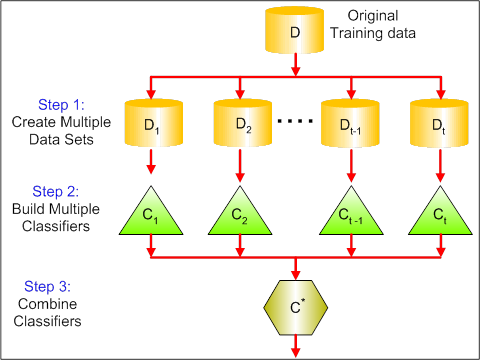
\includegraphics[width=\textwidth]{figures/external/bagging.png}
                \end{figure}
            \end{column}
        \end{columns}
    \end{frame}
    
    \begin{frame}{Random Forest}
        \begin{itemize}
            \item The objective behind \textbf{random forests} is to take a \textbf{set of high-variance, low-bias decision trees} and transform them into a \textbf{single model that has both low variance and low bias} by \textbf{aggregating the various outputs} of individual decision trees. Through \textbf{majority voting}, we can find the \textbf{average output given by most of the individual trees}.
            \item Instead of just simply averaging the predictions of the trees, which would make them just a forest, a random forest uses \textbf{two key concepts} that gives it the name random: \textbf{random sampling of training instances} when building trees and \textbf{random subsets of features} considered when splitting nodes.
            \item This element of \textbf{randomness} ensures that the decision tree learners create trees that are \textbf{not correlated with one another}. As a result, \textbf{potential errors are evenly spread throughout the model and are cancelled out by the majority voting} decision strategy of the model.
        \end{itemize}
    \end{frame}
    
    \begin{frame}{Random Training Subsets}
        \begin{columns}
            \begin{column}{0.6\textwidth}
                \begin{itemize}
                    \item When training, \textbf{each tree} in a random forest \textbf{learns from a random samples} that are \textbf{drawn with replacement}, known as \textbf{bootstrapping}, which means that \textbf{some samples will be used multiple times in a single tree}.
                    \item By training each tree on different samples, although each tree might have \textbf{high variance with respect to a particular set of the training data}, overall, the \textbf{entire forest will have lower variance but not at the cost of increasing the bias}.
                    \item The procedure of training each individual learner on different \textbf{bootstrapped subsets} of the data and then \textbf{averaging the predictions} is known as \textbf{bagging} or \textbf{bootstrap aggregating}.
                \end{itemize}
            \end{column}
            \begin{column}{0.4\textwidth}
                \begin{figure}
                    \label{fig:random-forest-1}
                    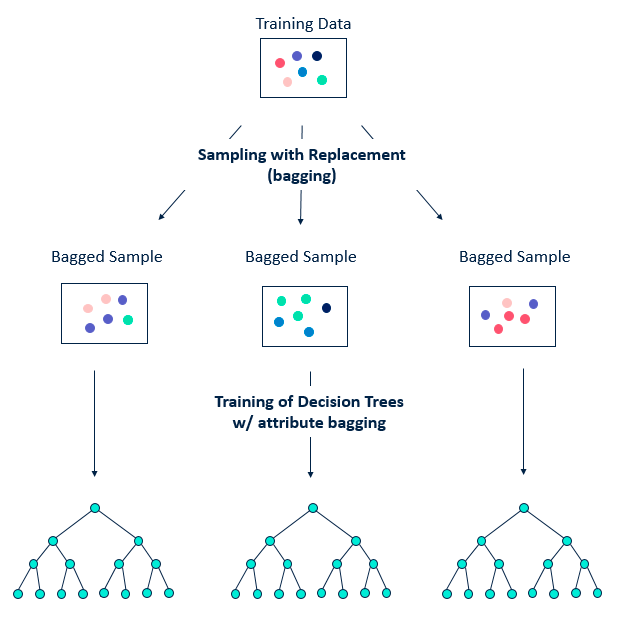
\includegraphics[width=\textwidth, cframe=gray]{figures/external/random-forest-2.png}
                \end{figure}
            \end{column}
        \end{columns}
    \end{frame}
    
    \begin{frame}{Random Feature Subsets}
        \begin{columns}
            \begin{column}{0.6\textwidth}
                \begin{itemize}
                    \item The other main concept in the random forest is that \textbf{only a subset of all the features} are considered for splitting each node in each decision tree. 
                    \item Generally this is set to $\sqrt{n\_features}$ for classification meaning that if there are \textbf{16 features}, at each node in each tree, \textbf{only 4 random features} will be considered for splitting the node.
                    \item The reason why subsampling features can further decorrelate trees is, that if there are \textbf{few dominating features}, these features \textbf{will be selected in many trees} even for \textbf{different subsamples}, making the \textbf{trees in the forest similar} (correlated) again.
                \end{itemize}
            \end{column}
            \begin{column}{0.4\textwidth}
                \begin{figure}
                    \label{fig:random-forest-2}
                    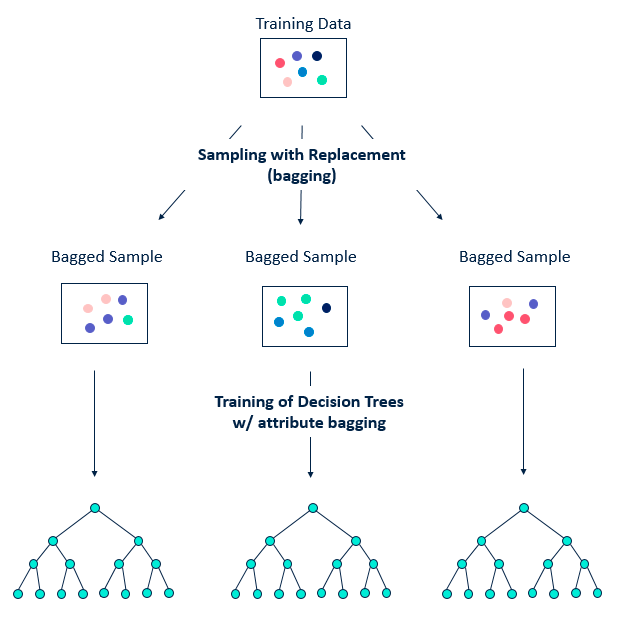
\includegraphics[width=\textwidth, cframe=gray]{figures/external/random-forest-2.png}
                \end{figure}
            \end{column}
        \end{columns}
    \end{frame}

    \begin{frame}{Python Implementation: Random Forest}
        \lstinputlisting[language=Python, style=material]{snippets/outage-rf-1.py}
    \end{frame}

    \begin{frame}{Predictive Maintenance Problem Result (Random Forest}
        \begin{figure}
            \label{fig:outages-rf-decision-tree}
            \includegraphics[height=0.8\textheight, keepaspectratio]{figures/outages-rf-decision-tree.pdf}
        \end{figure}
    \end{frame}

    \begin{frame}{Python Implementation: Random Forest Evaluation}
        \lstinputlisting[language=Python, style=material]{snippets/outage-rf-2.py}

        Baseline performance from ID3: 100\%/91.67\%.
    \end{frame}

    \begin{frame}{Hyperparameter Space}
        \begin{itemize}
            \item The random forest as a \textbf{more sophisticated model} than a basic decision tree made the results even worse. This might be not surprising due to the \textbf{large number of hyperparameters} a random forest brings with making the \textbf{hyperparameter space} to choose from when setting up the model incredibly huge.
            \item A single decision tree lets us choose from what \textbf{splitting criterion to use \textit{(criterion)}}, what the \textbf{maximum depth of the tree \textit{(max\_depth)}} should be, what \textbf{minimum number of samples are required to split an internal node \textit{(min\_samples\_split)}} any many many more.
            \item The random forest brings in even more hyperparameters to choose from like the number of trees in the forest \textit{(n\_estimators)}, the \textbf{number of features to consider when looking for the best split \textit{(max\_features)}} or whether \textbf{bootstrap samples should be used when building trees \textit{(bootstrap)}}.
            \item So far, we have been using the \textbf{default hyperparameters} for linear and logistic regression models as well as for decision trees and random forests as we did not know how to come up with the right hyperparameters for a specific problem.
        \end{itemize}

            
    \end{frame}

    \begin{frame}{Hyperparameter Tuning}
        The concepts of \textbf{overfitting, cross-validation and the bias-variance tradeoff} turn out to be \textbf{central to do a good job at optimizing the hyperparameters of algorithms} but how do we know the right values?

        \begin{figure}
            \label{fig:hyperparameter-tusdning}
            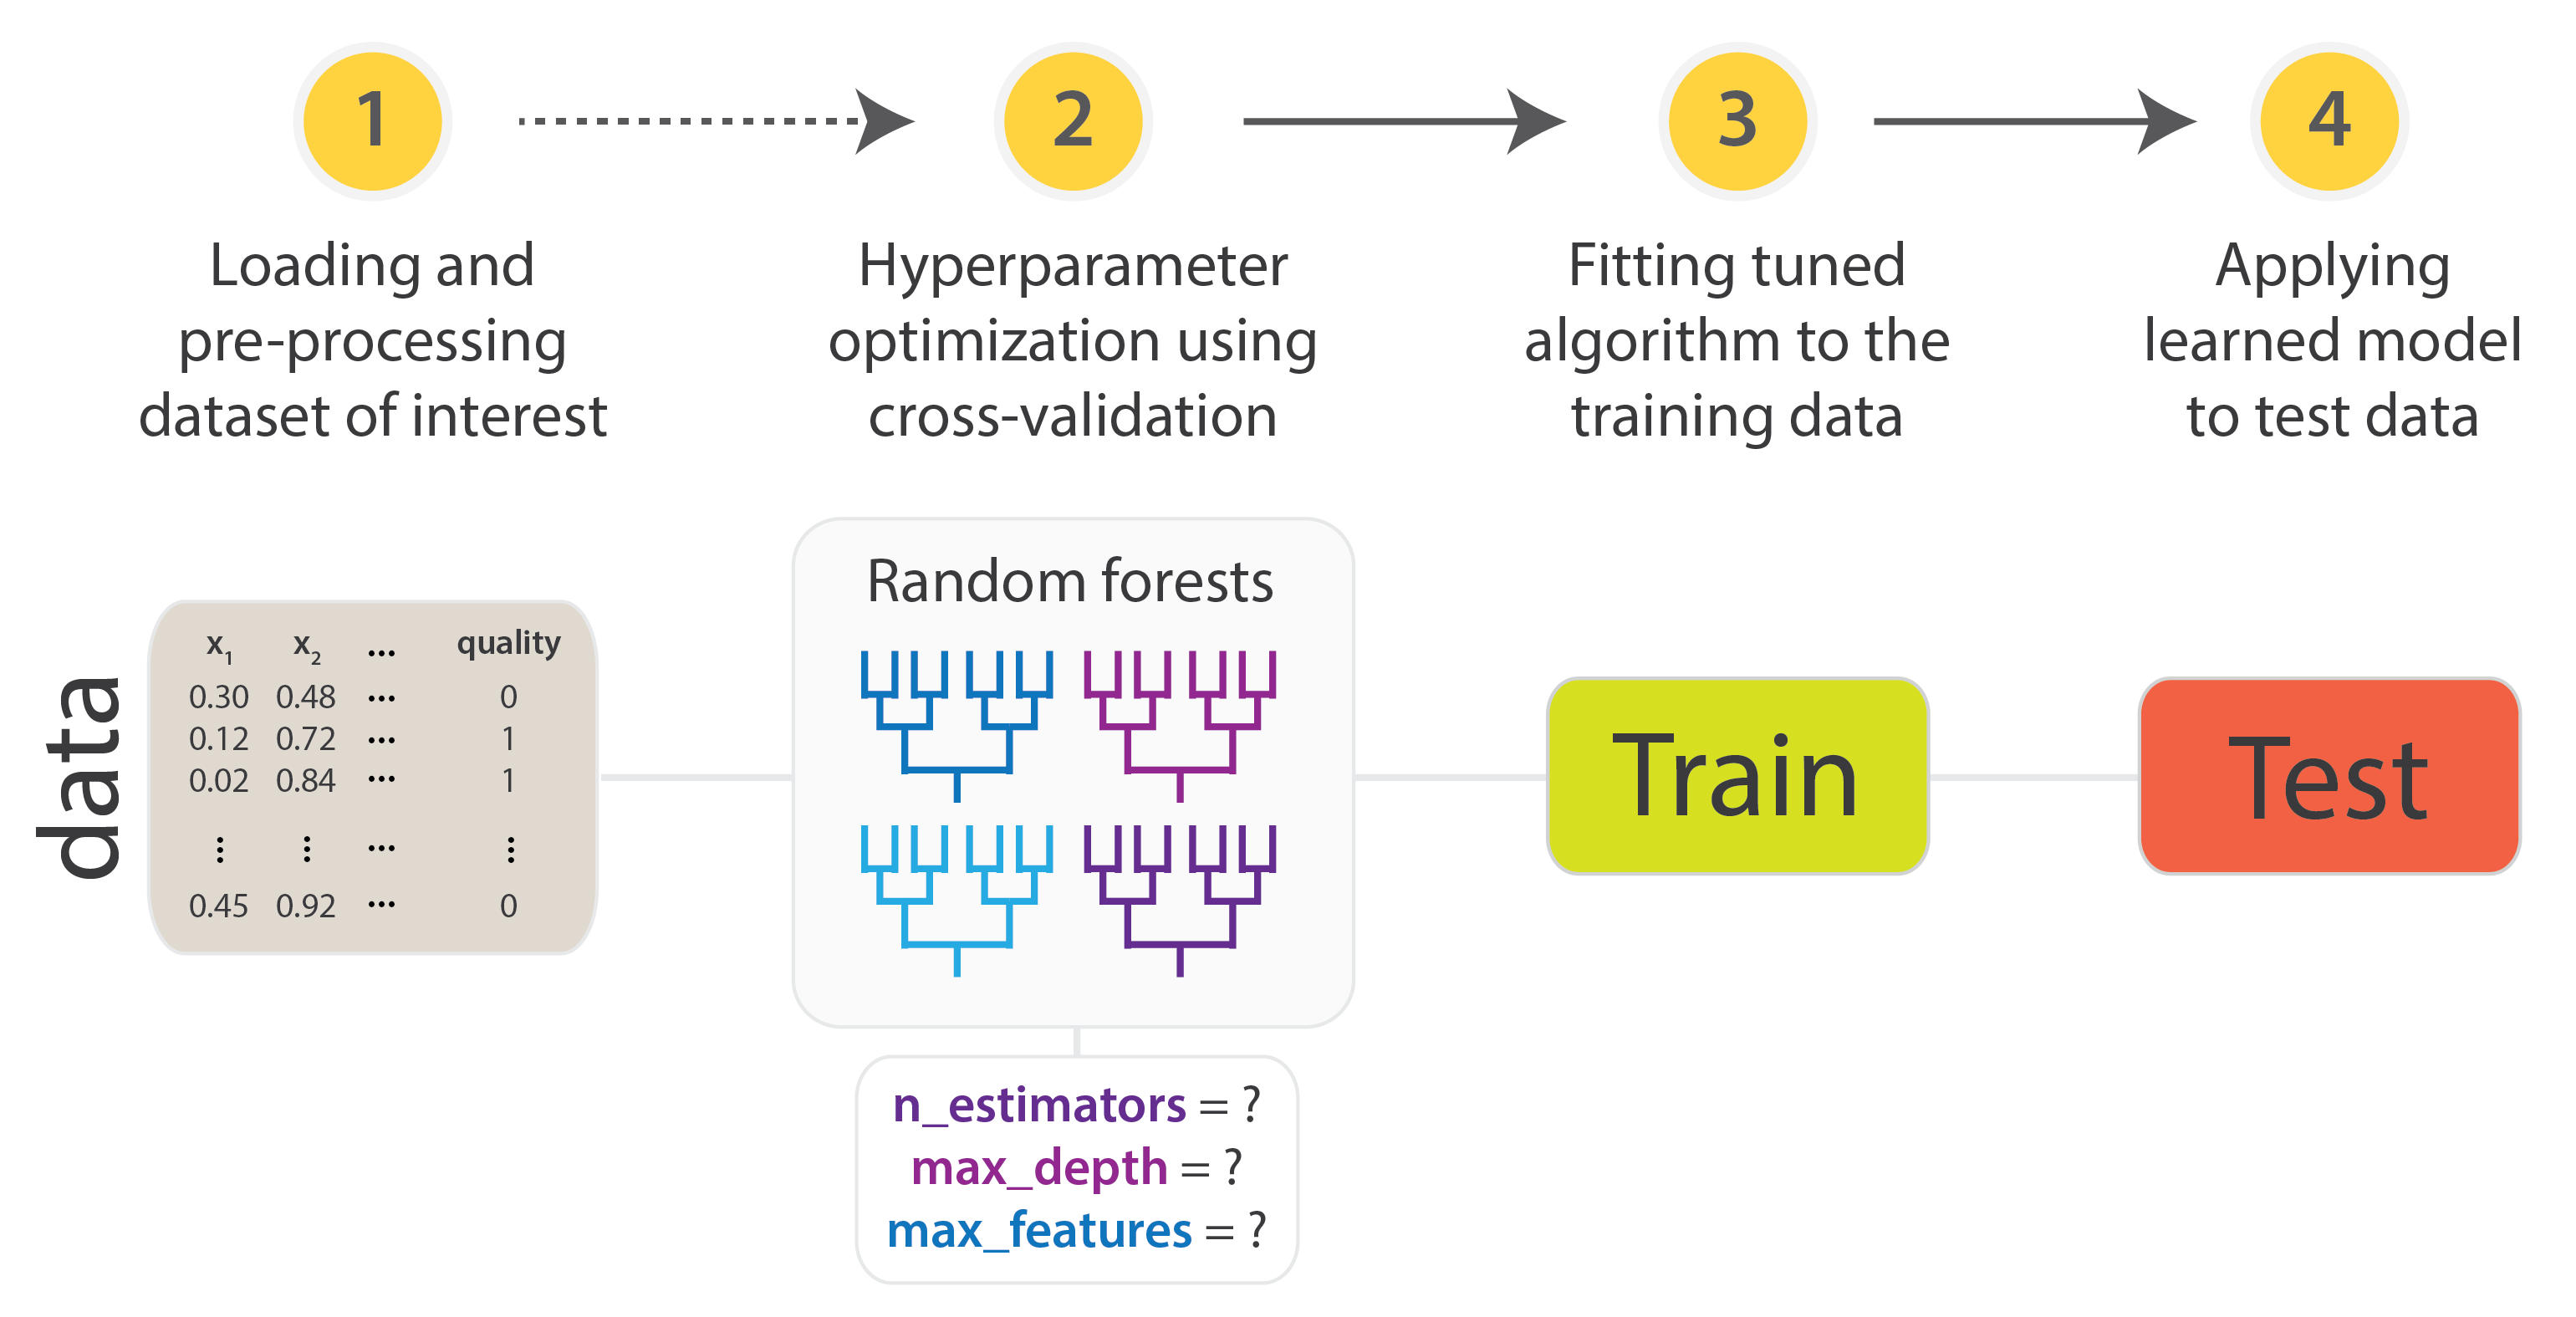
\includegraphics[width=0.5\textwidth]{figures/external/hyperparameter-tuning.png}
        \end{figure}

        \textbf{Hyperparameter tuning (or optimization)} exactly works the way one would expect - \textbf{trying out different hyperparameter values and see what works best}. However, we need make sure that the results getting \textbf{validated out-of-sample} and therefore \textbf{strategies to systematically explore the hyperparameter space}.
    \end{frame}

    \begin{frame}{Grid Search}
        \begin{columns}
            \begin{column}{.6\textwidth}
               \begin{itemize}
                    \item One strategy is the \textbf{grid search} which \textbf{exhaustively tries out all combinations of manually predefined hyperparameter values} together with a \textbf{k-fold cross-validation} and reports the best option, hence the name grid.
                    \item The benefit of this strategy is that \textbf{various combinations getting thoroughly tested out} but when it comes to \textbf{dimensionality} it can become impractical because the \textbf{number of evaluations (size of the search grid) increases exponentially with each additional hyperparameter} making it computationally expensive.
                    \item Therefore, to be tractable, the \textbf{number of combinations often have to be restricted} which can severely \textbf{limit how well the hyperparameter space is explored} and thus could lead to overlooking those regions in the hyperparameter space where the accuracy for example would be highest.
                \end{itemize}
            \end{column}
            \begin{column}{.4\textwidth}
                \begin{figure}
                    \label{fig:grid-search}
                    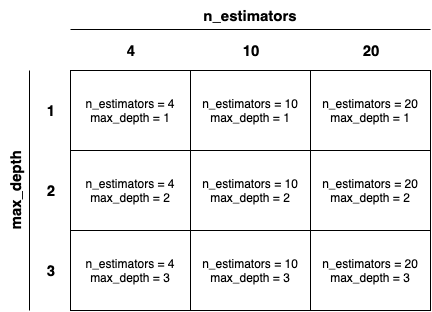
\includegraphics[width=\textwidth]{figures/drawio/grid-search.png}
                \end{figure}
            \end{column}
        \end{columns}
    \end{frame}
    
    \begin{frame}{Python Implementation: Grid Search}
        \lstinputlisting[language=Python, style=material]{snippets/outage-grid-search.py}
    \end{frame}

    \begin{frame}{Grid Search Iterations}
        \lstinputlisting[language=Python, style=material]{snippets/outage-grid-result-1.py}
    \end{frame}

    \begin{frame}{Randomized Search}
        \begin{columns}
            \begin{column}{.6\textwidth}
               \begin{itemize}
                    \item In \textbf{randomized search}, hyperparameter values are getting \textbf{sampled} a certain number of times from some \textbf{predefined distribution} which could be for example a \textbf{standard normal distribution} or a \textbf{uniform distribution} over some range.
                    \item What \textbf{kind of distribution} is appropriate depends on \textbf{what is reasonable and what is likely to be good}.
                    \item Lets assume a \textbf{hyperparameter space is 12x12} giving \textbf{144 possible combinations} of two hyperparameters. For testing 3 close values of each hyperparameter, \textbf{grid search} would need \textbf{9 iterations} to test out all combinations where \textbf{randomized search} for the same number of iterations would have \textbf{explored a space 16 times bigger}.
                    \item Only \textbf{one additional hyperparameter} would increase the \textbf{number of possibilities to search through up to 1728} making \textbf{randomized search the only feasible practical approach}.
                \end{itemize}
            \end{column}
            \begin{column}{.4\textwidth}
                \begin{figure}
                    \label{fig:hyperparameter-tuning-matrix}
                    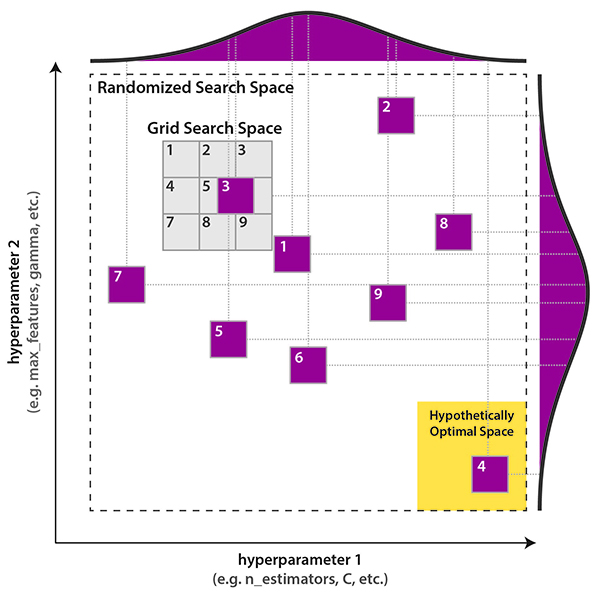
\includegraphics[width=\textwidth, cframe=gray]{figures/external/hyperparameter-tuning-matrix.jpg}
                \end{figure}
            \end{column}
        \end{columns}
    \end{frame}

    \begin{frame}{Python Implementation: Randomized Search}
        \lstinputlisting[language=Python, style=material]{snippets/outage-random-search.py}
    \end{frame}

    \begin{frame}{Randomized Search Iterations}
        \lstinputlisting[language=Python, style=material]{snippets/outage-random-search-result.py}
    \end{frame}

    \begin{frame}{Python Implementation: Randomized Search Hyperparameter Optimized Random Forest}
        \lstinputlisting[language=Python, style=material]{snippets/outage-rf-final.py}
    \end{frame}

    \begin{frame}[fragile]{Regression Counterpart}
        Of course, random forests are also suitable for \textbf{regression problems} by using a \verb|RandomForestRegressor| instead of a \verb|RandomForestClassifier| like follows:

        \begin{lstlisting}[language=Python, style=material]
# Additional Import Definitions
from sklearn.ensemble import RandomForestRegressor

# Model Initialization
model = RandomForestRegressor(**hyperparams)
        \end{lstlisting}

        A random forest for regression problems uses the \textbf{mean squared error} to measure the quality of a split and tries to minimizes the \textbf{L2 loss function} using the mean of each terminal node. To incorporate this, remember to set the hyperparameter \verb|criterion| to \verb|mse| instead of \verb|entropy|.
    \end{frame}

    \stepcounter{openexercise}
    \begin{frame}{Open Exercise \arabic{openexercise}}
        How do the \textbf{number of estimators of a random forest} and the \textbf{maximum depth of its corresponding trees} would \textbf{affect the bias and variance tradeoff}?
        \note{
            \textbf{The more trees (or estimators) the better!} Adding trees to a random forest \textbf{decreases overfitting which means less variance while not increasing the bias} thanks to bagging and random feature selection. However, increasing the number of estimators increases the computational costs.

            Limiting the maximum depth of decision trees, a r\textbf{andom forest can no more fit the training data} as closely and therefore the \textbf{variance is decreasing} but at the same time the \textbf{bias is increasing} as it may \textbf{not be able to capture certain patterns anymore}.

        }
    \end{frame}

    \stepcounter{devexercise}
    \begin{frame}{Development Exercise \arabic{devexercise}}
        \begin{alertblock}{\textsc{Task}}
            Import the \textbf{product backorders dataset} \textit{(datasets $\rightarrow$ exercises $\rightarrow$ backorders.csv)} into a notebook and learn an appropriate \textbf{random forest model} on the target \textit{went\_on\_backorder}. \textbf{Normalize all numeric and one-hot encode all categorical features} and perform a \textbf{randomized grid search} for both the \textbf{number of estimators sampled from a uniform distribution with a range from 200 to 400} and the \textbf{maximum depth of trees sampled from a uniform distribution with a range from 75 to 125}. Also set the random state to 1909.
        \end{alertblock}
        \begin{alertblock}{\textsc{Question}}
            Will a \textbf{product} with following attributes will \textbf{go on backorder} within the next 3 month and what is the probability estimate? Also report the \textbf{model performance} with an \textbf{appropriate metric} using a \textbf{10-fold cross-validation}!
            \begin{table}
                \scalebox{.8}{\begin{tabular}{m{2cm}m{2cm}m{2cm}m{2cm}m{2cm}}
\toprule
 national\_inv &  in\_transit\_qty &  forecast\_3\_month &  forecast\_6\_month &  forecast\_9\_month \\
\midrule
          100 &               0 &                 2 &                 5 &                 6 \\
\bottomrule
\end{tabular}
}

                \scalebox{.8}{\begin{tabular}{m{2cm}m{2cm}m{2cm}m{2cm}m{2cm}}
\toprule
 sales\_1\_month &  sales\_3\_month &  sales\_6\_month &  sales\_9\_month & ppap\_risk \\
\midrule
             1 &              2 &              5 &              1 &        no \\
\bottomrule
\end{tabular}
}
            \end{table}
        \end{alertblock}
        \note{
            Average F1 on Training and Test Sets: 97.38\%/89.74\%\\
            Prediction: array(['no'], dtype=object) \\
            Probability estimates: array([[0.80758017, 0.19241983]])
            
            \small{\href{https://nbviewer.jupyter.org/github/saschaschworm/big-data-and-data-science/blob/master/notebooks/development-exercises/backorder-random-forest.ipynb}{\textsc{\textbf{$\rightarrow$ open notebook in github}}}}

        }
    \end{frame}
       
    \begin{frame}{Summary: Decision Trees Models}
        \begin{alertblock}{\textsc{Task and Type}}
            Supervised Machine Learning Model for Regression and Classification Tasks
        \end{alertblock}
        \begin{alertblock}{\textsc{Performance Measure}}
            RMSE, Accuracy, Precision, Recall, F1, Area Under ROC Curve, Confusion Matrix
        \end{alertblock}
        \begin{alertblock}{\textsc{Strengths}}
            Decision trees can learn non-linear relationships and are able to naturally model non-linear decision boundaries thanks to their hierarchical structure; they are fairly robust to outliers and scalable; perform very well in practice, winning many classical (i.e. non-deep-learning) machine learning competitions;
        \end{alertblock}
        \begin{alertblock}{\textsc{Weaknesses}}
            Unconstrained, individual trees are prone to overfitting because they can keep branching until they memorize the training data, but this can be alleviated by ensemble methods.
        \end{alertblock}
    \end{frame}
\end{document}